\appendix

\section{Experimental Details}
\label{app:experimental-details}

This appendix provides the complete simulator, data-generation,
architecture, training, evaluation, and ablation details for
Section~\ref{sec:experiments}. The simulator is a controlled
mechanism-isolation environment rather than a calibrated model of a
specific disease.

\subsection{Controlled Medical Dynamical System}
\label{app:simulator}

\subsubsection{State and transition equations}

The simulator state is
\begin{equation}
    S_t=(X_t,C_t,D_t,U_t,A_{t-1}),
\end{equation}
where $X_t$ is the primary outcome, $C_t$ is a time-varying
clinical covariate and treatment-effect modifier, $D_t$ is decaying
cumulative treatment exposure, $U_t$ is an observed nuisance variable,
and $A_{t-1}$ is lagged treatment. For binary treatment
$A_t\in\{0,1\}$, the system evolves as
\begin{align}
    D_{t+1}
    &=0.72D_t+A_t,
    \label{eq:app-dose}\\
    C_{t+1}
    &=0.64C_t+0.13X_t+0.14A_t+\epsilon_t^C,
    \label{eq:app-covariate}\\
    U_{t+1}
    &=0.88U_t+\epsilon_t^U.
    \label{eq:app-nuisance}
\end{align}
The primary outcome evolves according to
\begin{align}
    X_{t+1}
    &=0.66X_t+0.18C_t+0.08\sin(X_t) \nonumber\\
    &\quad-\left(0.24+0.10\tanh(C_t)\right)A_t \nonumber\\
    &\quad+0.10A_{t-1}-0.055D_t+\epsilon_t^X.
    \label{eq:app-outcome}
\end{align}
The process noises are mutually independent with
\begin{equation}
    \epsilon_t^X,\epsilon_t^C,\epsilon_t^U
    \sim\mathcal N(0,0.04^2).
\end{equation}
Initial states are sampled as
\begin{align}
    X_0&\sim\mathcal N(0,0.75^2), &
    C_0&\sim\mathcal N(0,0.65^2),\\
    U_0&\sim\mathcal N(0,1).&&
\end{align}
with $D_0=0$ and initial lagged treatment sampled from
$\operatorname{Bernoulli}(0.4)$.

The primary outcome is $Y_t=X_t$. The model predicts
$V_t=(X_t,C_t)$ because $C_t$ affects both subsequent outcome dynamics
and treatment response. $D_t$ is not directly supplied as an input
feature, but is deterministically recoverable from the observed action
history through Equation~\eqref{eq:app-dose}.

\subsubsection{Design rationale}

\begin{table*}[t]
\centering
\small
\caption{Purpose of each simulator component.}
\label{tab:simulator-rationale}
\begin{tabular}{lll}
\toprule
Component & Role in the system & Failure mode tested \\
\midrule
$X_t$ & Primary clinical outcome & Outcome and effect-trajectory accuracy \\
$C_t$ & Time-varying effect modifier & Loss of treatment-relevant information \\
$D_t$ & Decaying cumulative exposure & Memory and cumulative treatment response \\
$A_{t-1}$ & Delayed treatment term & Propagation beyond immediate action effects \\
$U_t$ & Persistent nuisance & Capacity allocated to effect-irrelevant variation \\
State-dependent assignment & Observational treatment policy & Latent realization under identifiable confounding \\
Non-linear response & Mild $\sin$ and $\tanh$ terms & Non-linear rather than purely linear fitting \\
\bottomrule
\end{tabular}
\end{table*}

The autoregressive coefficients are below one to keep trajectories
stable. Treatment, lag, and cumulative-exposure effects are chosen to be
detectable without dominating the state dynamics. The coefficients are
not intended as estimates for a real disease.

\subsection{Observational Assignment and Identification}
\label{app:assignment}

Training trajectories are generated under the historical treatment
assignment mechanism
\begin{equation}
\begin{aligned}
    P(A_t=1\mid H_t)
    =\sigma(&-0.45+0.85X_t+0.65C_t\\
            &+0.35A_{t-1}-0.08D_t),
\end{aligned}
\label{eq:app-propensity}
\end{equation}
where $\sigma$ is the logistic function. The policy mimics the fact that
clinical treatment depends on current state and prior exposure rather
than being independently randomized. All variables influencing both
treatment and future outcome are contained in the complete observed
history, with $D_t$ reconstructible from prior actions. Sequential
exchangeability is therefore imposed by construction at the full-history
level. The logistic assignment maintains non-zero probability for both
actions over the realized state range. These assumptions establish
identifiability in the simulator; they are not claimed to hold
automatically in observational clinical data.

\subsection{Data Generation and Splits}
\label{app:data-generation}

Training data are generated online rather than stored as a fixed cohort.
At each of 600 gradient-update steps, we draw a fresh minibatch of 96
trajectories from the historical data-generating process. Each trajectory
contains a 16-step observed context followed by 8 factual future
transitions. Training is therefore specified in optimization steps, not
epochs over a fixed dataset: each model is exposed to $600\times96=57{,}600$
fresh trajectory windows. For a given seed, the one-step, multi-step, and
Temporal JEPA objectives receive the same sequence of factual training
batches.

After the 600th update, we retain the final checkpoint; we do not perform
early stopping or choose among intermediate checkpoints. For every seed,
we then freeze the trained model and generate 768 new observational
validation trajectories. Validation performs no backpropagation or
parameter update, and validation trajectories are not merged into the
training data. We report diagnostics at horizons
$\{1,2,4,8,16\}$, while model selection uses only the horizon-8 observed
rollout and latent-closure errors described in
Appendix~\ref{app:model-selection-details}. After selecting
$\lambda_J=1$, we evaluate the corresponding originally trained
checkpoints without retraining.

Final counterfactual testing uses a third, disjoint sample of 768 initial
patient histories, each with a 16-step observed context. Within a seed,
all methods use the same validation trajectories, test histories, and
treatment schedules, enabling paired comparisons. Random-number streams
for training, observational validation, and counterfactual testing are
disjoint. Counterfactual outcomes and treatment-effect errors are never
used for training, checkpoint selection, or hyperparameter selection.

During counterfactual testing, future process noise is set to zero and
both treatment branches begin from the identical simulated patient state.
The resulting contrast is the conditional-mean treatment response of the
known system rather than a contrast contaminated by independent future
noise draws.

\subsection{World Model and Optimization}
\label{app:model-details}

Each history token contains
\begin{equation}
    (X_s,C_s,U_s,A_{s-1},r_s),
\end{equation}
where $r_s$ is the normalized position within the 16-step context window,
linearly increasing from $-1$ to $0$. This feature is distinct from the
trajectory length $T$. The five-dimensional token is projected to model
dimension 32 and added to a fixed sinusoidal positional encoding. It is
then processed by a two-layer pre-norm Transformer encoder with four
attention heads, feed-forward width 96, ReLU activation, and dropout
$0.05$. The final token representation is linearly compressed to
$Z_t\in\mathbb R^{d_z}$.

The residual action-conditioned transition is
\begin{equation}
    \widehat Z_{t+1}
    =\widehat Z_t
    +0.25f_\theta([\widehat Z_t,A_t]),
\end{equation}
where $f_\theta$ is an MLP with input width $d_z+1$, hidden width 64,
$\tanh$ activation, and output width $d_z$. The factor $0.25$ scales the
residual update. The decoder is an MLP
$d_z\rightarrow64\rightarrow2$ with a $\tanh$ hidden activation and
outputs $(\widehat X,\widehat C)$. Unless otherwise stated, $d_z=8$.
Table~\ref{tab:architecture-hyperparameters} gives the complete fixed
configuration.

\begin{table}[t]
\centering
\caption{World-model architecture and optimization settings shared by
all main methods.}
\label{tab:architecture-hyperparameters}
\small
\setlength{\tabcolsep}{4pt}
\begin{tabular}{ll}
\toprule
Component & Setting \\
\midrule
Observed context & 16 steps \\
Factual training horizon & 8 steps \\
Token features & $(X,C,U,A_{s-1},r_s)$ \\
Transformer layers & 2 \\
Model dimension & 32 \\
Attention heads & 4 \\
Transformer FFN width & 96 \\
Transformer activation & ReLU \\
Transformer dropout & 0.05 \\
Normalization & pre-norm \\
Latent dimension & $d_z=8$ \\
Transition MLP & $(d_z+1)\rightarrow64\rightarrow d_z$ \\
Transition activation & $\tanh$ \\
Residual scale & 0.25 \\
Outcome decoder & $d_z\rightarrow64\rightarrow2$ \\
Decoder activation & $\tanh$ \\
Optimizer & AdamW \\
Learning rate & $8\times10^{-4}$ \\
Weight decay & $10^{-4}$ \\
Gradient clipping & norm 1 \\
Batch size & 96 \\
Optimization budget & 600 updates \\
Random seeds & $\{0,1,2,3,4\}$ \\
\bottomrule
\end{tabular}
\end{table}

The one-step baseline supervises only $h=1$. Multi-step prediction and
Temporal JEPA supervise observable outcomes at every horizon
$h=1,\ldots,8$, using linearly increasing weights from 1 to 1.5.
Temporal JEPA additionally matches normalized online and target
representations at $\mathcal H_J=\{1,2,4,8\}$. The target encoder is
initialized as a copy of the online encoder, receives no gradients, and
is updated after each optimization step by EMA with momentum $m=0.99$.
We train $\lambda_J\in\{0.1,1,10\}$ and select it using observational
validation only. The backbone configuration, $\mathcal H_J$, and $m$
are fixed for the main comparison; alternatives are reported as
sensitivity analyses in Appendix~\ref{app:ablation-details}. Every
reported neural result aggregates five seeds $\{0,1,2,3,4\}$.

\subsection{Treatment Schedules and Effect Evaluation}
\label{app:schedules}

Let $\bar 0_{16}$ denote no treatment for 16 future steps. We compare it
with the schedules in Table~\ref{tab:schedules}. The label
\texttt{seen\_block} is retained in the released code for historical
reasons; it denotes a behavior-like early block, not a claim that the
exact 16-step sequence was explicitly supplied as a training policy.
None of the four fixed schedules is supplied as an explicit training
regime. Training actions are sampled step by step from the historical
state-dependent assignment mechanism. Consequently, local action
subsequences may occur during training even though the complete fixed
schedule is held out as a training policy. We therefore describe this as
temporal composition rather than strict out-of-support extrapolation.

\begin{table}[t]
\centering
\caption{Prespecified horizon-16 evaluation schedules.}
\label{tab:schedules}
\begin{tabular}{ll}
\toprule
Schedule & Treated future steps \\
\midrule
No treatment & none \\
Early block & $\{0,1,2,3\}$ \\
Alternating & $\{0,2,4,6,8,10,12,14\}$ \\
Separated & $\{0,4,8,12\}$ \\
Late-separated & $\{3,7,11,15\}$ \\
\bottomrule
\end{tabular}
\end{table}

For patient $i$ and schedule $\bar a$, the true and predicted effects
relative to no treatment are
\begin{align}
    \tau_{i,h}(\bar a,\bar 0)
    &=X_{i,t+h}(\bar a)-X_{i,t+h}(\bar 0),\\
    \widehat\tau_{i,h}(\bar a,\bar 0)
    &=\widehat X_{i,t+h}(\bar a)
      -\widehat X_{i,t+h}(\bar 0).
\end{align}
The reported horizon-$H$ effect MSE averages the squared difference
between these two quantities over patients and all steps $1,\ldots,H$.
It is therefore an individual effect-trajectory error in this controlled
deterministic evaluation, rather than squared error between two
population-average effects.

We additionally report two absolute trajectory metrics. For the primary
outcome,
\begin{equation}
    \mathcal R_X^{(H)}(\bar a)
    =\frac{1}{NH}\sum_{i=1}^{N}\sum_{h=1}^{H}
    \left(\widehat X_{i,t+h}(\bar a)-X_{i,t+h}(\bar a)\right)^2.
\end{equation}
For the joint observed state $V_t=(X_t,C_t)$,
\begin{equation}
    \mathcal R_V^{(H)}(\bar a)
    =\frac{1}{2NH}\sum_{i=1}^{N}\sum_{h=1}^{H}
    \left\|\widehat V_{i,t+h}(\bar a)-V_{i,t+h}(\bar a)\right\|_2^2.
\end{equation}
Both are evaluated under all five schedules, including no future
treatment. Treatment-effect MSE is evaluated for the four intervention
schedules relative to the common no-treatment branch. All primary test
results use $H=16$.

\subsection{Latent Information Probes}
\label{app:latent-probes}

For $d_z\in\{1,2,4,8,16\}$, five factual multi-step models are trained.
Each model is frozen before collecting latent states. Ridge probes predict
$X_t$, $C_t$, $D_t$, and $U_t$; a linear score predicts binary lagged
treatment and is evaluated by ROC--AUC. For each model, 4,000 latent
states are collected, with 70\% used to fit the probes and 30\% reserved
for evaluation. Continuous variables are evaluated by test $R^2$. Probe
performance diagnoses linear recoverability only: it does not establish
that the transition makes functional use of the decoded information.

\begin{table*}[t]
\centering
\small
\caption{Latent-capacity diagnosis. Entries are means over five seeds.
Factual and effect errors are unscaled MSE; continuous probes report
test $R^2$, and the lagged-treatment probe reports ROC--AUC.}
\label{tab:latent-probes}
\begin{tabular}{crrrrrrr}
\toprule
$d_z$ & Factual & H16 effect & $X_t$ $R^2$ & $C_t$ $R^2$
& $D_t$ $R^2$ & $U_t$ $R^2$ & $A_{t-1}$ AUC \\
\midrule
1  & 0.002760 & 0.007176 & 0.927 & 0.073 & 0.780 & 0.002 & 0.781 \\
2  & 0.002691 & 0.002813 & 0.929 & 0.908 & 0.957 & $-0.000$ & 0.944 \\
4  & 0.002505 & 0.002012 & 0.936 & 0.939 & 0.968 & 0.282 & 0.964 \\
8  & 0.002267 & 0.002238 & 0.953 & 0.959 & 0.972 & 0.856 & 0.979 \\
16 & 0.002212 & 0.003962 & 0.991 & 0.985 & 0.980 & 0.976 & 1.000 \\
\bottomrule
\end{tabular}
\end{table*}

The $d_z=1$ model retains $X_t$ but largely loses the effect modifier
$C_t$, despite a factual MSE close to the $d_z=2$ model. Increasing
capacity restores treatment-relevant variables but also makes the
effect-irrelevant nuisance $U_t$ recoverable. The non-monotone effect MSE
shows that recoverability and capacity alone do not certify intervention
fidelity.

\subsection{Transition Diagnosis}
\label{app:transition-diagnosis}

The transition diagnosis uses 45 fitted models: 25 factual multi-step
models with $d_z\in\{1,2,4,8,16\}$, five $d_z=8$ models trained under
balanced treatment assignment, and 15 $d_z=8$ models trained with local
treatment-contrast weights $1$, $10$, or $100$. Each configuration uses
five seeds. Starting from an observed history, we apply pulse, four-step
block, and alternating schedules for 16 steps.
At horizons $\{0,1,2,4,8,16\}$, we compare
\begin{enumerate}
    \item the rolled state obtained through recursive transition; and
    \item the encoded state obtained by re-encoding the corresponding
    true future history.
\end{enumerate}
Both states are evaluated using the same model-implied one-step treatment
response. The amplification ratio is
\begin{equation}
    \operatorname{Amp}_h
    =
    \frac{\operatorname{MSE}
    (\widehat\tau_{\mathrm{rolled},h},\tau_h)}
    {\operatorname{MSE}
    (\widehat\tau_{\mathrm{encoded},h},\tau_h)+10^{-12}}.
\end{equation}
This diagnostic separates information available after encoding the true
history from information retained after recursive latent transition.
For the alternating schedule at $H=16$, the median amplification across
the 45 models is $4.82$; $68.9\%$ exceed a factor of two and $48.9\%$
exceed a factor of five. These summaries are computed across fitted
models rather than across individual patients.

\subsection{Model Selection}
\label{app:model-selection-details}

On observational validation trajectories, the rollout criterion is
\begin{equation}
    \mathcal R_{\mathrm{obs}}^{(H)}
    =\frac{1}{2NH}\sum_{i=1}^{N}\sum_{h=1}^{H}
    \left\|\widehat V_{i,t+h}^{\mathrm{obs}}
    -V_{i,t+h}^{\mathrm{obs}}\right\|_2^2.
\end{equation}
The closure criterion compares the recursively rolled state with the
same online encoder applied directly to the corresponding observed
future history:
\begin{equation}
    \mathcal R_{\mathrm{cl}}^{(H)}
    =\frac{1}{Nd_z}\sum_{i=1}^{N}
    \left\|\operatorname{norm}(\widehat Z_{i,t+H})
    -\operatorname{norm}(E_\phi(H_{i,t+H}))\right\|_2^2.
\end{equation}
Both quantities are computable without counterfactual outcomes.

For each $\lambda_J\in\{0.1,1,10\}$, we average observational validation
metrics across five seeds. With prediction horizon $H_p=8$, closure
horizon $H_c=8$, and tolerance $\gamma=1.10$, the
eligible set is
\begin{equation}
    \mathcal M_{\mathrm{eligible}}
    =\left\{M:
    \mathcal R_{\mathrm{pred}}^{\mathrm{val}}(M)
    \leq
    \gamma\mathcal R_{\mathrm{pred}}^{\mathrm{val}}
    (M_{\mathrm{multi}})
    \right\}.
\end{equation}
The multi-step baseline has validation MSE $0.003497$, producing a
ceiling of $0.003847$. JEPA weights $0.1$ and $1$ are eligible, whereas
$10$ is not. Their closure MSEs are $0.001749$ and $0.000384$, so the
rule selects $\lambda_J=1$. The selection is made at the configuration
level; all five seeds are retained for final reporting.

\begin{table}[t]
\centering
\caption{JEPA-weight selection at $H_p=H_c=8$. Validation and final
effect MSE are multiplied by $10^3$. The effect column is reported only
after selection and is not used by the rule.}
\label{tab:app-lambda-selection}
\scriptsize
\setlength{\tabcolsep}{3pt}
\begin{tabular}{cccccc}
\toprule
$\lambda_J$ & Obs. & Clos. & Elig. & Sel. & Effect \\
\midrule
0.1 & 3.596 & 1.749 & Yes & No  & 1.263 \\
1   & 3.673 & 0.384 & Yes & Yes & 1.360 \\
10  & 3.985 & 0.143 & No  & No  & 2.266 \\
\bottomrule
\end{tabular}
\end{table}

The final test effect happens to be lowest at $\lambda_J=0.1$. We do not
use this fact to revise the selected model because the corresponding
counterfactual quantity is unavailable in observational validation and
using it would leak the synthetic test target into model selection.

\subsection{Ablation and Sensitivity Details}
\label{app:ablation-details}

Training-design ablations use $\lambda_J=1$ and five seeds. We compare
JEPA horizons $\{1\}$, $\{8\}$, and $\{1,2,4,8\}$, and EMA momentum
$m\in\{0,0.9,0.99,0.999\}$. Selection sensitivity is recomputed without
retraining for $H_c\in\{1,2,4,8,16\}$ and
$\gamma\in\{1.00,1.05,1.10,1.20\}$. No counterfactual metric is used to
choose a configuration in any sensitivity analysis.

\begin{table*}[t]
\centering
\caption{Temporal JEPA training ablations. Observed rollout and closure
are measured at $H=8$ on observational validation trajectories. Effect
MSE averages the four horizon-16 test contrasts. Values are means over
five seeds, multiplied by $10^3$.}
\label{tab:app-jepa-ablation}
\begin{tabular}{lccc}
\toprule
Variant & H8 observed & H8 closure & H16 mean effect \\
\midrule
JEPA $\{1\}$, $m=0.99$ & 3.689 & 15.626 & 1.404 \\
JEPA $\{8\}$, $m=0.99$ & 3.774 & 2.437 & 1.543 \\
JEPA $\{1,2,4,8\}$, $m=0$ & 4.014 & 0.719 & 1.905 \\
JEPA $\{1,2,4,8\}$, $m=0.9$ & 3.690 & 0.453 & \textbf{1.289} \\
JEPA $\{1,2,4,8\}$, $m=0.99$ & \textbf{3.673} & \textbf{0.384} & 1.360 \\
JEPA $\{1,2,4,8\}$, $m=0.999$ & 3.705 & 0.498 & 1.849 \\
\bottomrule
\end{tabular}
\end{table*}

The horizon ablation changes only the JEPA matching set
$\mathcal H_J$; every variant retains observable prediction supervision
at all steps $1,\ldots,8$. The full set $\{1,2,4,8\}$ achieves the
lowest observed, closure, and mean effect errors among the horizon
variants. For EMA, both $m=0.9$ and $m=0.99$ improve over no momentum,
whereas $m=0.999$ degrades effect accuracy. The main configuration keeps
the standard $m=0.99$ setting rather than retuning on test effects.

\begin{table}[t]
\centering
\small
\caption{Prediction-gate sensitivity at selection horizon $H_c=8$.
The gate is $\mathcal R_{\mathrm{obs}}\leq
\gamma\mathcal R_{\mathrm{obs}}(M_{\mathrm{multi}})$.}
\label{tab:app-gate-sensitivity}
\begin{tabular}{ccc}
\toprule
$\gamma$ & Eligible JEPA weights & Selected weight \\
\midrule
1.00 & none & none \\
1.05 & $0.1$ & $0.1$ \\
1.10 & $0.1,1$ & $1$ \\
1.20 & $0.1,1,10$ & $10$ \\
\bottomrule
\end{tabular}
\end{table}

\begin{table}[t]
\centering
\small
\caption{Sensitivity to closure-selection horizon at the main gate
$\gamma=1.10$.}
\label{tab:app-horizon-sensitivity}
\begin{tabular}{cc}
\toprule
$H_c$ & Selected weight \\
\midrule
1 & $0.1$ \\
2 & $1$ \\
4 & $1$ \\
8 & $1$ \\
16 & $10$ \\
\bottomrule
\end{tabular}
\end{table}

\begin{figure*}[t]
    \centering
    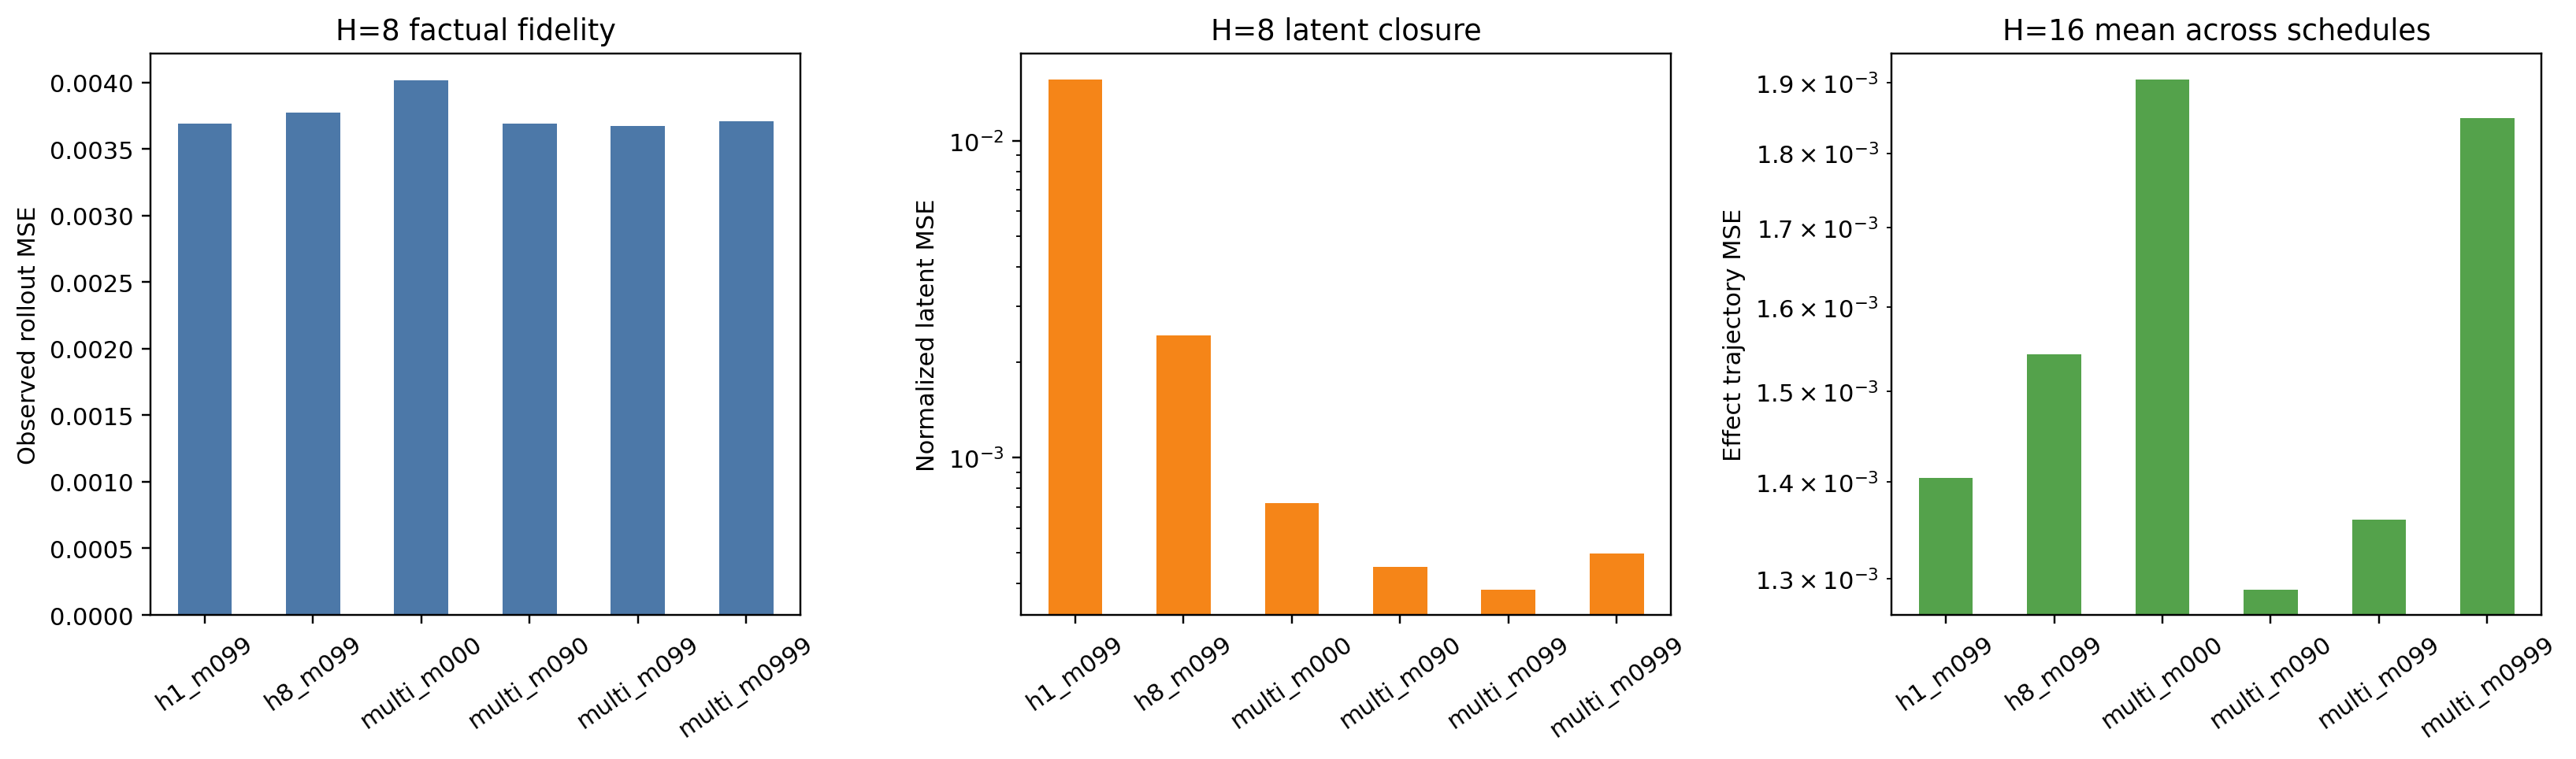
\includegraphics[width=0.97\textwidth]
    {figures/temporal_jepa_ablation/temporal_jepa_ablation.png}
    \caption{Training-design ablations. Multi-horizon matching strongly
    improves closure, while treatment-effect performance is non-monotonic
    in both closure and EMA momentum.}
    \label{fig:jepa-ablation}
\end{figure*}

\subsection{Reproducibility and Released Artifacts}

All experiments are implemented in the accompanying repository. The
latent-capacity study is reproduced by
\texttt{scripts/run\_medical\_latent.py}; transition amplification by
\texttt{scripts/run\_transition\_diagnosis.py}; the main Temporal JEPA
experiment by \texttt{scripts/run\_temporal\_jepa.py}; absolute
interventional trajectories by
\texttt{scripts/evaluate\_interventional\_trajectories.py}; and the
training and selection ablations by
\texttt{scripts/run\_temporal\_jepa\_ablation.py}. Per-seed CSV files,
aggregate summaries, and figure-generation outputs are retained under
\texttt{results/} and \texttt{figures/}. Random seeds and all reported
hyperparameters are stored with the released results.

\subsection{Additional Limitations of the Controlled Evaluation}

The system contains only one calibrated level of noise and one family of
state-dependent treatment assignment mechanisms. The main method is
tested with one small Transformer architecture, so the experiments do
not establish architecture-independent gains. Moreover, the evaluation
schedules are not supplied as explicit training policies, but the
stochastic observational generator does not guarantee that every short
subsequence is absent from training. Finally, causal identification is
assumed by construction. The experiments therefore evaluate how a finite
latent world model realizes identifiable effects; they do not solve
unmeasured confounding or lack of treatment support in real clinical
data.
